\documentclass[12pt,a4paper]{article}
\usepackage[utf8]{inputenc}
\usepackage[T1]{fontenc}
\usepackage{lmodern}
\usepackage[spanish,es-tabla]{babel}
\usepackage{graphicx} % Sin [demo] para que cargue tu diagrama real
\usepackage{geometry}
\usepackage[hidelinks]{hyperref}
\usepackage{float}
\usepackage{xcolor}
\usepackage{titlesec}
\usepackage{tcolorbox}
\usepackage{tabularx}
\usepackage{amssymb}
\usepackage{colortbl}
\usepackage{enumitem}
\usepackage{fancyhdr}

% Configuración de márgenes (headheight ajustado para corregir el warning de fancyhdr)
\geometry{top=2.5cm, bottom=2.5cm, left=2.5cm, right=2.5cm, headheight=25pt}
\setlength{\parskip}{0.4em}

% Colores Institucionales EPN / ATA
\definecolor{epnblue}{RGB}{15, 52, 96} % Azul oscuro institucional
\definecolor{epngold}{RGB}{212, 175, 55} % Dorado/Amarillo
\definecolor{graytext}{RGB}{80, 80, 80}

% Formateo de Títulos (Serif para coincidir con el template)
\titleformat{\section}{\Large\bfseries\color{epnblue}}{\thesection.}{0.5em}{}[\titlerule]
\titleformat{\subsection}{\large\bfseries\color{epnblue}}{\thesubsection}{0.5em}{}

% Diseño de Cajas de Alerta y Notas
\tcbuselibrary{skins,breakable}
\newtcolorbox{warningbox}[1][]{
    enhanced,
    frame hidden,
    breakable,
    colback=gray!10,
    borderline west={3pt}{0pt}{red!80!black},
    fonttitle=\bfseries\color{red!80!black},
    coltitle=red!80!black,
    title=ADVERTENCIA,
    attach title to upper=\quad,
    boxsep=3pt,
    left=6pt,
    right=6pt,
    top=6pt,
    bottom=6pt,
    #1
}

\newtcolorbox{infobox}[1][]{
    enhanced,
    frame hidden,
    breakable,
    colback=gray!5,
    borderline west={3pt}{0pt}{epnblue},
    fonttitle=\bfseries\color{epnblue},
    coltitle=epnblue,
    title=NOTA,
    attach title to upper=\quad,
    boxsep=3pt,
    left=6pt,
    right=6pt,
    top=6pt,
    bottom=6pt,
    #1
}

% Configuración de Encabezados y Pies de Página
\pagestyle{fancy}
\fancyhf{}
\fancyhead[L]{\textcolor{epnblue}{\small Plataforma Cuadricóptero - Cube Black}}
\fancyhead[R]{\textcolor{graytext}{\small Manual operativo}}
\fancyfoot[C]{\thepage}
\renewcommand{\headrulewidth}{0.5pt}
\renewcommand{\headrule}{\hbox to\headwidth{\color{epnblue}\leaders\hrule height \headrulewidth\hfill}}

\begin{document}

% ---------------------------------------------------------
% PORTADA INSTITUCIONAL (TEMPLATE ATA / EPN)
% ---------------------------------------------------------
\begin{titlepage}
    \centering
    
    % Encabezado Institucional
    \vspace*{1cm}
    \textcolor{epnblue}{\rule{\textwidth}{1pt}}\\[0.3cm]
    \textcolor{epnblue}{\textsc{\Large Escuela Politécnica Nacional}}\\[0.15cm]
    \textcolor{graytext}{\small Facultad de Ingeniería Mecánica}\\[0.1cm]
    \textcolor{graytext}{\small Grupo de Investigación en Aeronáutica y Termofluidos Aplicados}\\[0.2cm]
    \textcolor{epnblue}{\rule{\textwidth}{0.5pt}}
    
    \vspace{2.5cm}
    
    % Título del Documento
    \textcolor{epnblue}{\Large \bfseries Manual de configuración y operación}\\[0.2cm]
    \textcolor{epnblue}{\Large \bfseries Plataforma Cuadricóptero de Entrenamiento}\\[0.2cm]
    \textcolor{epnblue}{\Large \bfseries Controlador Cube Black}
    
    \vspace{1cm}
    
    % Separador Dorado
    \textcolor{epngold}{\rule{4cm}{1pt}}
    
    \vspace{1cm}
    
    % Badge Manual Operativo (CON PADDING AJUSTADO)
    {\setlength{\fboxsep}{12pt}%
    \colorbox{epnblue}{\textcolor{white}{\enskip \textbf{MANUAL OPERATIVO} \enskip}}}
    
    \vspace{2cm}
    
    % Metadatos
    \begin{table}[H]
        \centering
        \small
        \renewcommand{\arraystretch}{1.3}
        \begin{tabular}{rl}
            \textbf{Autores:} & Victor Humberto Cruz Armijos \\
            \textbf{Institución:} & Escuela Politécnica Nacional (EPN) \\
            \textbf{Departamento:} & Facultad de Ingeniería Mecánica \\
            \textbf{Área de investigación:} & Monitoreo de ecosistemas altoandinos \\
            \textbf{Fecha:} & Septiembre de 2026 \\
            \textbf{Clasificación:} & Manual técnico interno \\
            \textbf{Versión:} & 1.0 \\
        \end{tabular}
    \end{table}
    
    \vfill
    
    % Pie de página portada
    \textcolor{epnblue}{\rule{\textwidth}{1pt}}\\[0.2cm]
    \textcolor{graytext}{\scriptsize Quito, Ecuador - Ladrón de Guevara E11-253 - www.epn.edu.ec}
    
\end{titlepage}

% ---------------------------------------------------------
% ÍNDICE Y RESUMEN
% ---------------------------------------------------------
\newpage
\tableofcontents
\newpage

\begin{abstract}
El presente documento detalla el procedimiento técnico paso a paso como reporte final para la reconstrucción del chasis, configuración electrónica y de software de un vehículo aéreo no tripulado (cuadricóptero) utilizando un controlador de vuelo de la familia Cube (ej. Cube Black) con firmware ArduPilot, emisora Flysky FS-i6X y los softwares de estación terrena (QGroundControl y Mission Planner). Se documentan las observaciones descubiertas durante el ensamblaje, resolución de problemas de hardware, integración de módulos GNSS de precisión, telemetría avanzada, sintonización de PID en vuelo y protocolos operativos de seguridad civil para su despliegue en ecosistemas altoandinos.
\end{abstract}

\vspace{1cm}

\section*{Advertencias de Seguridad y Disclaimer}
\addcontentsline{toc}{section}{Advertencias de Seguridad y Disclaimer}

\begin{warningbox}[title=Precauciones Críticas de Seguridad Operativa]
La operación de Vehículos Aéreos No Tripulados (VANT) conlleva riesgos inherentes de carácter material y físico que el operador debe mitigar preventivamente.
\begin{itemize}[leftmargin=*]
    \item \textbf{Riesgo Eléctrico e Ignición:} Las baterías de Polímero de Litio (LiPo) son altamente volátiles si se perforan, cortocircuitan o sobrecargan. Se debe utilizar siempre bolsas ignífugas (\textit{LiPo Safe Bags}) para su transporte y proceso de carga.
    \item \textbf{Riesgo Mecánico (Hélices):} Las hélices rígidas girando a altas revoluciones pueden causar laceraciones graves. \textbf{Nunca} se debe armar el equipo ni conectar la batería principal en espacios cerrados sin retirar previamente las hélices de los motores.
    \item \textbf{Responsabilidad del Operador:} El ensamblador y piloto asumen total responsabilidad por daños a terceros. El presente manual es una guía técnica y no exime al operador de cumplir con la normativa de la Dirección General de Aviación Civil (DGAC).
\end{itemize}
\end{warningbox}

\newpage

% ---------------------------------------------------------
% NUEVA SECCIÓN: INTRODUCCIÓN Y CONCEPTOS BÁSICOS
% ---------------------------------------------------------
\section{Introducción y Conceptos Básicos}

\subsection{Propósito del Manual}
El presente documento ha sido elaborado bajo los estándares del Grupo de Investigación en Aeronáutica y Termofluidos Aplicados (ATA), con el objetivo de servir como guía integral para los nuevos investigadores y operadores. Establece los procedimientos estandarizados para el ensamblaje, configuración en la estación terrena y vuelo seguro de la plataforma de entrenamiento (cuadricóptero) impulsada por el controlador Cube Black.

\subsection{Arquitectura del Sistema de Control}
El vuelo de una aeronave de ala rotatoria es inherentemente inestable y depende de un lazo de control cerrado ejecutado cientos de veces por segundo:
\begin{enumerate}[leftmargin=*]
    \item \textbf{Sensores (IMU y GNSS):} Las Unidades de Medición Inercial (acelerómetros y giroscopios) leen la inclinación y aceleración del dron, mientras que el módulo GPS determina su posición absoluta.
    \item \textbf{Controlador de Vuelo (Cube Black):} Procesa los datos de los sensores mediante el filtro EKF (Extended Kalman Filter) y los compara con los comandos deseados por el piloto (enviados a través del receptor de radio).
    \item \textbf{Controladores PID:} El software calcula el error entre la posición actual y la deseada, generando una señal de corrección.
    \item \textbf{Actuadores (ESC y Motores):} Los Variadores de Velocidad (ESC) traducen la señal de corrección en modulación de pulsos trifásicos (PWM), ajustando instantáneamente las revoluciones (RPM) de cada motor para estabilizar la aeronave.
\end{enumerate}

\subsection{Dinámica de Vuelo (Ejes Espaciales)}
Para operar el equipo y comprender las gráficas de telemetría, es vital dominar los tres ejes de rotación:
\begin{itemize}[leftmargin=*]
    \item \textbf{Roll (Alabeo):} Inclinación lateral (izquierda o derecha). Controla el desplazamiento horizontal lateral.
    \item \textbf{Pitch (Cabeceo):} Inclinación frontal o trasera. Controla el avance o retroceso de la aeronave.
    \item \textbf{Yaw (Guiñada):} Rotación sobre su propio eje vertical. Cambia la dirección hacia donde apunta la nariz del dron.
    \item \textbf{Throttle (Acelerador):} Control de la potencia general enviada a los cuatro motores simultáneamente para ganar o perder altitud.
\end{itemize}

\subsection{Proyección Tecnológica: Plataformas VTOL}
Las configuraciones detalladas en este manual para el cuadricóptero sientan las bases matemáticas y procedimentales para operar vehículos más complejos. En aeronaves VTOL (Vertical Take-Off and Landing), el controlador Cube Black utilizará los mismos principios de sintonización PID (Roll, Pitch, Yaw) descritos aquí para estabilizar la aeronave durante el despegue vertical. Una vez ganada la altitud, el Autopiloto ejecutará la "transición" hacia el vuelo aerodinámico tradicional (ala fija), apagando los motores de sustentación y activando el motor de empuje frontal.

\section{Lista de Componentes del Sistema y Ubicación Estratégica}
A continuación, se detalla el hardware principal utilizado para la reconstrucción y configuración de este vehículo aéreo, priorizando el aislamiento electromagnético:

\begin{itemize}[leftmargin=*]
    \item \textbf{Controlador de Vuelo:} Autopiloto Cube Black integrado en su placa portadora (Carrier Board estándar).
    \item \textbf{Motores:} Motores Brushless (HobbyPower / equivalentes a AIR 2213 de 1000KV). 
    \item \textbf{Sistema de Radiocontrol:} Emisora Flysky FS-i6X sincronizada con un receptor FS-iA10B (operando bajo protocolo digital puro i-BUS).
    \item \textbf{Sistema de Navegación:} Módulo Here GNSS, que incluye receptor de satélites y magnetómetro (brújula) externo vía I2C.
    \item \textbf{Telemetría de Largo Alcance:} Módulos de radiofrecuencia (ej. RFD900 o similares) operando en 433/915 MHz.
    \item \textbf{Fuente de Alimentación:} Batería LiPo de 3 celdas (3S).
    \item \textbf{Actuadores Adicionales:} Variadores de Velocidad (ESC) de 20A y hélices de plástico con rotación CW y CCW.
    \item \textbf{Estructura:} Chasis central en configuración cuádruple, acoplado a un tren de aterrizaje compuesto por tubos de fibra de carbono (10 mm) y acoples de unión fabricados mediante impresión 3D (PETG/ABS).
\end{itemize}

\section{Observaciones de Ensamblaje: Precauciones de Hardware}

Durante la reconstrucción del chasis y las pruebas preliminares, se identificaron puntos críticos de fallo mecánico-eléctrico que deben evitarse estrictamente.

\subsection{Tornillería en Motores y Cortocircuitos}
Al fijar los motores brushless a la estructura o a los acoples impresos en 3D, la selección de la longitud de los tornillos es un factor de seguridad vital.

\begin{warningbox}[title=El Problema de los Cortocircuitos]
Un tornillo excesivamente largo penetrará la base del estator y perforará el esmalte aislante protector de las bobinas de cobre internas. Esto provoca un cortocircuito directo que viaja a través de la fibra de carbono (material conductivo), causando que el motor no gire, asimetrías de arranque o daños permanentes en los ESC. \textbf{Solución:} Siempre debe existir un espacio de separación (\textit{gap}) visible entre la punta del tornillo de sujeción y el bobinado del motor.
\end{warningbox}

\section{Configuración del Enlace de Radio (Hardware)}

\subsection{Diferenciación de Enlaces (Telemetría vs. Control)}
Es fundamental separar físicamente el enlace de datos (telemetría) del enlace de radiocontrol.
\begin{itemize}[leftmargin=*]
    \item \textbf{Telemetría:} Transmite datos MAVLink a la estación terrena (433/915 MHz). Se conecta a los puertos \texttt{TELEM 1} o \texttt{TELEM 2} de la placa portadora.
    \item \textbf{Radiocontrol:} Transmite los comandos de vuelo (2.4 GHz). Se conecta al puerto \texttt{RC IN} del Cube.
\end{itemize}

\subsection{Conexión del Receptor Flysky FS-iA10B (Protocolo i-BUS)}
Para evitar la latencia e interferencias del protocolo analógico PPM y omitir la inversión innecesaria de S.BUS, se configura el sistema en el estándar digital nativo de Flysky: \textbf{i-BUS}.
\begin{enumerate}[leftmargin=*]
    \item \textbf{Selección de Puerto en el Receptor:} Se debe utilizar \textbf{únicamente} el puerto horizontal superior etiquetado como \texttt{SERVO} dentro del bloque de salida de datos. Este puerto emite la trama digital pura de los 10 canales.
    \item \textbf{Polaridad:} Se debe respetar el orden lógico de los pines:
    \begin{itemize}
        \item \textbf{Señal (S):} Hacia el interior de la placa del receptor (cable amarillo o blanco).
        \item \textbf{Voltaje (+):} Pin central (5V, cable rojo).
        \item \textbf{Tierra (-):} Hacia el borde exterior de la placa (cable café o negro).
    \end{itemize}
    \item \textbf{Verificación de Energía:} Al conectar el puerto USB al Cube, este alimenta al receptor. El LED rojo debe encenderse de forma fija, indicando vinculación correcta con la emisora.
\end{enumerate}

\subsection{Conexiones Centrales del Controlador Cube}
El bloque central de conexiones maneja la distribución de energía y las señales PWM hacia los variadores de velocidad. El diagrama general de la arquitectura del hardware se detalla a continuación:

\begin{figure}[H]
    \centering
    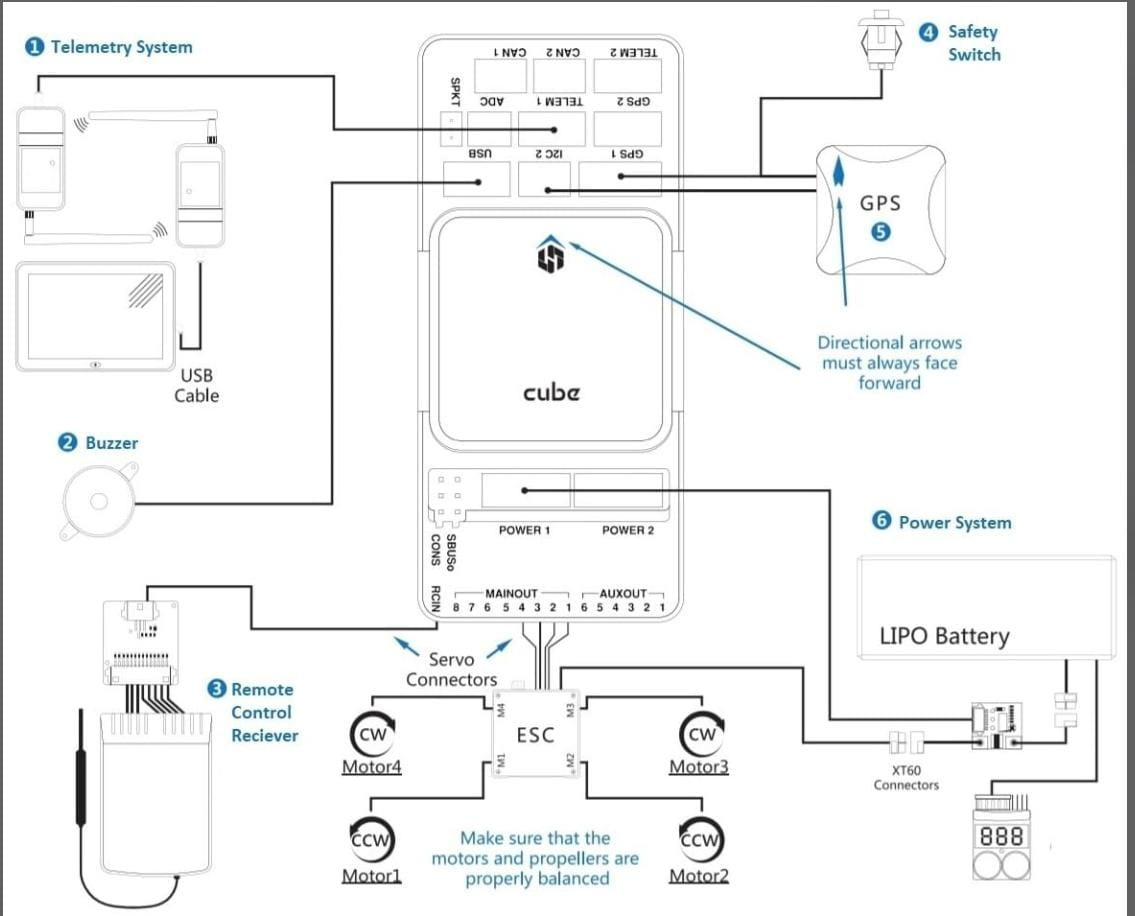
\includegraphics[width=0.95\textwidth]{Diagrama_dron.jpeg}
    \caption{Diagrama general de conexiones del controlador Cube, ilustrando la integración del sistema de telemetría, zumbador (buzzer), receptor RC, módulo GPS y la distribución de potencia hacia los ESC.}
\end{figure}

\section{Configuración del Protocolo en la Emisora}
Para que la emisora envíe la información en formato digital sin inversiones lógicas por el puerto SERVO, se debe configurar estrictamente en modo i-BUS.
\begin{enumerate}[leftmargin=*]
    \item Mantener presionado el botón \texttt{OK} de la Flysky FS-i6X para acceder al menú principal.
    \item Navegar a \texttt{System Setup} $\rightarrow$ \texttt{RX Setup} $\rightarrow$ \texttt{Output Mode}.
    \item Seleccionar la salida como \textbf{PWM \& i-BUS} (o \textbf{Serial: i-BUS} según el firmware). Evitar S.BUS.
    \item \textbf{Guardado:} Mantener presionado el botón \texttt{CANCEL} durante 3 segundos para grabar la configuración.
\end{enumerate}

\section{Conexión al Software y Parámetros de Comunicación}
Para enlazar el controlador Cube a las estaciones terrenas (Mission Planner o QGroundControl), es mandatorio configurar la velocidad de transmisión (\textit{Baud Rate}) adecuada según el medio físico:
\begin{itemize}[leftmargin=*]
    \item \textbf{Conexión alámbrica (Cable USB):} Seleccionar el puerto COM correspondiente y configurar la velocidad estándar de ArduPilot a \textbf{115200} baudios.
    \item \textbf{Conexión inalámbrica (Telemetría):} Cuando se utilizan módulos de radiofrecuencia (ej. RFD900 o RFD900x), la velocidad obligatoria en la estación terrena debe ajustarse a \textbf{57600} baudios. Se recomienda selección manual, ya que la función "Auto" presenta fallos en enlaces de radio.
\end{itemize}

\section{Configuración Avanzada de Telemetría (Radios RFD900 / SiK)}
Para misiones autónomas o vuelos donde el dron excede la línea de visión directa (BVLOS), la estabilidad del enlace de datos a 915 MHz o 433 MHz es crítica.

\subsection{Emparejamiento (Pairing) y Ajuste de Potencia}
Para que el radio de tierra (conectado por USB a la computadora) y el radio del aire (en el dron) se comuniquen, deben estar estrictamente emparejados. Esto se puede realizar mediante programas externos dedicados o directamente en Mission Planner:
\begin{enumerate}[leftmargin=*]
    \item En Mission Planner, conectar vía USB al radio local (No al dron).
    \item Dirigirse a \texttt{Setup} $\rightarrow$ \texttt{Optional Hardware} $\rightarrow$ \texttt{SiK Radio}.
    \item Hacer clic en \textbf{Load Settings}. Aparecerán dos columnas: la configuración del radio local y la del radio remoto.
    \item \textbf{Emparejamiento (Net ID):} El parámetro crítico es el \textbf{Net ID} (Identificador de Red). Ambos radios deben poseer exactamente el mismo número (ej. \texttt{25}). Si los números difieren, los módulos se ignorarán mutuamente.
    \item \textbf{Regulación Termal:} Reducir el valor de \textbf{Tx Power} (medido en dBm) si las pruebas se realizan en laboratorio. Transmitir a 30 dBm (1 Vatio) en distancias cortas puede quemar el módulo de radio o saturar el receptor. Para vuelos cortos, de 14 a 20 dBm es suficiente. Presionar \textit{Save Settings}.
\end{enumerate}

\begin{infobox}[title=Monitoreo del Enlace (RSSI)]
El RSSI (\textit{Received Signal Strength Indicator}) es el parámetro vital que debe revisarse en el HUD de Mission Planner durante el vuelo. Valores cercanos a \textbf{200} indican una señal excelente. Si el valor cae por debajo de \textbf{50-60} constantemente, existe un riesgo inminente de desconexión y pérdida del enlace (GCS Failsafe).
\end{infobox}

\section{Sincronización de ESC y Configuración de Arranque}
Para garantizar un despegue estable y simétrico, los variadores de velocidad (ESC) deben memorizar los límites exactos de la señal de radio, eliminando zonas muertas de fricción.

\subsection{Ajuste de Energía Base (Ralentí) en Mission Planner}
Para definir el comportamiento de los motores al armar, se ajustan los umbrales de energía en la pestaña \textit{Full Parameter Tree}:
\begin{itemize}[leftmargin=*]
    \item \textbf{MOT\_SPIN\_ARM:} Energía base inyectada al armar. Se fija en \textbf{0.04} (4\%) para que los motores giren de forma continua y suave al recibir el comando de armado, confirmando su operatividad antes del despegue.
    \item \textbf{MOT\_SPIN\_MIN:} Velocidad mínima garantizada en vuelo. Se fija en \textbf{0.06} (6\%) estableciendo un límite inferior de seguridad para evitar paradas de motor durante descensos rápidos.
\end{itemize}

\subsection{Procedimiento de Calibración Masiva (Vía Software)}
Este método permite calibrar los cuatro variadores simultáneamente utilizando la señal central del Autopiloto.
\begin{enumerate}[leftmargin=*]
    \item \textbf{Preparación:} Con el dron desenergizado (sin batería conectada), conectar el Cube Black a la computadora mediante cable USB.
    \item \textbf{Activación en Mission Planner:} Dirigirse a \textit{Full Parameter Tree}, buscar el parámetro \texttt{ESC\_CALIBRATION}, cambiar su valor a \textbf{1} y presionar \textit{Write Params}.
    \item \textbf{Reinicio Obligatorio:} Desconectar el cable USB para apagar el Autopiloto por completo.
    \item \textbf{Aceleración Máxima:} Encender la emisora Flysky y subir la palanca izquierda (acelerador) al \textbf{100\%}.
    \item \textbf{Energización y Armado Forzado:} Conectar la batería LiPo principal. \textit{(Nota: Si el módulo GPS posee un botón físico de seguridad con luz roja parpadeante, mantenerlo presionado hasta que la luz quede fija para forzar el paso de la señal hacia los ESC).}
    \item \textbf{Confirmación de Límite Superior:} Los motores emitirán la melodía inicial de encendido, seguida inmediatamente de \textbf{dos pitidos agudos}, indicando que han registrado el valor máximo de la palanca.
    \item \textbf{Límite Inferior:} Bajar rápidamente la palanca del acelerador al \textbf{0\%}.
    \item \textbf{Guardado:} Los ESC emitirán un \textbf{pitido largo y sólido}, confirmando que el rango completo ha sido memorizado. Desconectar la batería.
\end{enumerate}

\subsection{Procedimiento de Calibración Individual (Alternativa CH3)}
Si la calibración masiva mediante el Autopiloto presenta asimetrías de encendido (como se detalla en el Anexo A), se debe aislar el hardware y calibrar de forma directa cada motor. Ejecutar el siguiente ciclo por cada uno de los cuatro motores:
\begin{enumerate}[leftmargin=*]
    \item Desconectar el cable de control (señal PWM) del ESC de la placa portadora del Cube.
    \item Conectar dicho cable del ESC directamente a los pines del \textbf{Canal 3 (CH3)} en el receptor Flysky FS-iA10B.
    \item Encender la emisora Flysky y subir la palanca izquierda (acelerador) al \textbf{100\%}.
    \item Conectar la batería LiPo principal al dron.
    \item Tras escuchar los \textbf{dos pitidos agudos} (límite superior), bajar rápidamente la palanca del acelerador al \textbf{0\%}.
    \item Esperar el \textbf{pitido largo y sólido} de confirmación y desconectar la batería.
    \item Repetir el proceso con el siguiente motor y, al finalizar, reconectar todos los ESC a sus puertos \texttt{MAIN OUT} correspondientes en el Cube.
\end{enumerate}

\section{Integración Avanzada de Módulos GNSS de Precisión (Here2)}
Una mala integración física o configuración espacial corromperá el filtro EKF y provocará incidentes de vuelo errático.

\subsection{Montaje Físico Estricto}
\begin{itemize}[leftmargin=*]
    \item \textbf{Orientación Direccional:} La flecha de la carcasa \textbf{debe apuntar exactamente} hacia el frente (nariz) del dron, paralela a la flecha del Cube Black. Una desviación forzará un vuelo en espiral (efecto \textit{Toilet Bowl}).
    \item \textbf{Aislamiento Magnético:} El GPS siempre debe instalarse sobre un mástil, alejado al menos 10 cm de la placa distribuidora de energía, motores y baterías.
\end{itemize}

\subsection{Diagnóstico de Errores I2C}
Los módulos Here clásicos o configurados de fábrica a menudo utilizan el bus I2C para el compás.
\begin{itemize}[leftmargin=*]
    \item \textbf{Bad Compass Health:} Problema de comunicación de hardware. Verificar que el cable de 4 pines esté correctamente asentado en el puerto \texttt{I2C 2} del Autopiloto.
    \item \textbf{Compass Variance:} Contradicción entre compás interno y externo. Priorizar siempre el externo en Mission Planner.
\end{itemize}

\subsection{Compensación Espacial (GPS Offset)}
Si el mástil del módulo GNSS no está fijado exactamente en el centro de gravedad (CG) matemático de la aeronave, el Autopiloto calculará mediciones inerciales erróneas. Mida la distancia en metros desde el centro del Cube Black hasta el centro del módulo GPS y configúrela en el \textit{Full Parameter Tree} respetando el sistema NED (North, East, Down):

\begin{warningbox}[title=La Trampa del Eje Z (Orientación NED)]
ArduPilot utiliza el estándar aeroespacial NED (North, East, Down). Esto significa que el eje Z es \textbf{positivo hacia abajo}. Como el GPS va montado en un mástil por encima de la placa, el valor Z debe ser estrictamente \textbf{negativo} (ej. \texttt{-0.15} si el mástil mide 15 cm). Ingresarlo en positivo empeorará severamente la navegación.
\end{warningbox}

\begin{itemize}[leftmargin=*]
    \item \textbf{GPS\_POS1\_X:} Distancia en el eje longitudinal. (Positivo si está desplazado hacia adelante; negativo si está hacia atrás).
    \item \textbf{GPS\_POS1\_Y:} Distancia en el eje lateral. (Positivo a la derecha; negativo a la izquierda).
    \item \textbf{GPS\_POS1\_Z:} Distancia en el eje vertical (Altitud). \textbf{Debe ser negativo}.
\end{itemize}

\section{Calibración de Sensores Inerciales}

\subsection{Calibración de la Radio}
\begin{enumerate}[leftmargin=*]
    \item Navegar a la pestaña \texttt{Radio} en Mission Planner. Las barras verdes deben responder al movimiento de las palancas de forma continua.
    \item Hacer clic en \textbf{Calibrate} y mover ambos \textit{joysticks} en círculos cubriendo sus límites mecánicos máximos.
    \item Mover todos los interruptores auxiliares de extremo a extremo. Guardar con \textbf{Done}.
\end{enumerate}

\subsection{Acelerómetro}
\begin{enumerate}[leftmargin=*]
    \item En la pestaña \texttt{Setup}, seleccionar \texttt{Accelerometer}.
    \item Establecer \texttt{Autopilot Rotation} en \textbf{None}.
    \item Ejecutar la calibración ubicando el cuadricóptero en las 6 orientaciones solicitadas, manteniéndolo completamente inmóvil durante la lectura en cada paso.
\end{enumerate}

\subsection{Compás (Brújula) y Módulo GPS Externo}
\begin{enumerate}[leftmargin=*]
    \item En la pestaña \texttt{Compass}, priorizar el compás externo (External) y desmarcar las brújulas internas si el ruido electromagnético es elevado.
    \item Proceder con \textit{Onboard Mag Calibration} rotando el dron sobre todos sus ejes.
    \item \textbf{Aprendizaje Dinámico:} Cambiar el parámetro \texttt{COMPASS\_LEARN} a \textbf{3} (InFlight) en el \textit{Full Parameter Tree} permite que el EKF compense dinámicamente las interferencias magnéticas residuales durante el vuelo.
    \item Reiniciar el controlador de vuelo (\textit{Reboot}).
\end{enumerate}

\section{Prevención de Interferencias Electromagnéticas (EMI)}

\subsection{Fuentes Generadoras de Campos Magnéticos (Alejar)}
\begin{itemize}[leftmargin=*]
    \item \textbf{Cables de Batería y PDB:} Los cables principales y la Placa de Distribución son los mayores generadores de ruido.
    \item \textbf{Variadores (ESC):} Deben montarse en los brazos del dron, por las altas corrientes que conmutan.
    \item \textbf{Motores Brushless:} Sus bobinas generan campos magnéticos perjudiciales para los sensores de navegación.
\end{itemize}

\subsection{Mejores Prácticas de Ensamblaje Estructural}
\begin{enumerate}[leftmargin=*]
    \item \textbf{Trenzado de Cables:} Trenzar los cables de alta corriente (positivo y negativo) ayuda a cancelar los campos magnéticos opuestos.
    \item \textbf{Ruteo de Señal:} Pasar los cables de comunicación por conductos separados de los cables de potencia para evitar inducción de corrientes parásitas.
\end{enumerate}

\section{Extracción y Análisis de Registros de Vuelo (DataFlash Logs)}
Para diagnosticar el rendimiento dinámico y la seguridad de la aeronave post-vuelo, es imperativo analizar la telemetría interna almacenada en la memoria del controlador.

\subsection{Descarga de Registros (Logs)}
\begin{enumerate}[leftmargin=*]
    \item Conectar el controlador de vuelo a Mission Planner mediante cable USB para evitar pérdida de paquetes.
    \item Navegar a la pestaña \textbf{DataFlash Logs}.
    \item Seleccionar \textbf{Download DataFlash Log Via Mavlink}, elegir el archivo \texttt{.bin} correspondiente a la sesión más reciente y guardarlo.
\end{enumerate}

\subsection{Análisis de Consumo de Batería y Eficiencia Energética}
Para calcular el rendimiento y prevenir apagados en el aire (\textit{Failsafe} prematuro), se deben validar los parámetros del módulo de potencia. En la lista derecha, despliega la categoría \textbf{BAT} y luego la subcarpeta \textbf{0}:
\begin{itemize}[leftmargin=*]
    \item \textbf{Corriente Consumida:} Graficar la variable \texttt{Curr}. En un vuelo estacionario ideal (Hover), este valor debe mantenerse estable. 
    \item \textbf{Caída de Voltaje (\textit{Voltage Sag}):} Graficar \texttt{Volt} (voltaje real) y observar la diferencia con \texttt{VoltR} (voltaje en reposo estimado). Una caída severa del voltaje real (mayor a 1.0V) al acelerar indica batería degradada.
    \item \textbf{Capacidad Total Consumida (mAh):} Graficar \texttt{CurrTot}. Este parámetro suma los miliamperios-hora extraídos a lo largo del vuelo. Si consume más del 80\% de la capacidad nominal en menos de 10 minutos, optimice el peso (MTOW).
\end{itemize}

\subsection{Diagnóstico del Filtro EKF y Anomalías Magnéticas}
\begin{itemize}[leftmargin=*]
    \item Graficar la variable \textbf{SM} (Compass Test Ratio) desplegando los núcleos \texttt{0} y \texttt{1} dentro de la categoría \textbf{XKF4}.
    \item \textbf{Criterio de Aceptación:} La curva graficada debe mantenerse constantemente por debajo del valor de \textbf{0.5}. Picos repentinos indican interferencia electromagnética severa.
\end{itemize}

\subsection{Análisis de Vibraciones Inerciales y Saturación (Clipping)}
\begin{itemize}[leftmargin=*]
    \item \textbf{Niveles de Aceleración:} Desplegar la categoría \textbf{VIBE} y graficar \texttt{VibeX}, \texttt{VibeY} y \texttt{VibeZ}. Promedios deben oscilar debajo de \textbf{30 m/s\textsuperscript{2}}.
    \item \textbf{Saturación (Clip):} Graficar \texttt{Clip0}, \texttt{Clip1} y \texttt{Clip2}. Deben permanecer estrictamente en \textbf{0} durante el vuelo. Incrementos indican resonancia de motores.
\end{itemize}

\subsection{Evaluación de Distribución de Carga Motriz (RCOUT)}
\begin{itemize}[leftmargin=*]
    \item Desplegar la categoría \textbf{RCOU} (Salida de Radio Control) y graficar conjuntamente las señales PWM \texttt{C1}, \texttt{C2}, \texttt{C3} y \texttt{C4}.
    \item Las cuatro líneas deben presentar un trazado compacto, entrelazado y agrupado (típicamente entre 1400 y 1600 ms).
    \item \textbf{Señal de Falla:} Una curva PWM significativamente más alta indica que dicho motor requiere girar a mayor velocidad para compensar un desbalance o rodamiento dañado.
\end{itemize}

\section{Optimización Avanzada de Control y Perfil de Vuelo}

\subsection{Aprendizaje Automático de Vuelo Estacionario (Hover)}
Para establecer una línea base precisa en los cálculos de navegación autónoma, el Autopiloto debe registrar la potencia motriz nominal del chasis.
\begin{enumerate}[leftmargin=*]
    \item Configurar la directiva \textbf{MOT\_HOVER\_LEARN} al valor \textbf{2} (\textit{Learn and Save}).
    \item Realizar un vuelo estacionario ininterrumpido en modo \textbf{Loiter} o \textbf{AltHold} durante un mínimo de 30 segundos.
    \item Tras aterrizar, el controlador de vuelo reescribirá automáticamente el parámetro \textbf{MOT\_THST\_HOVER} con el coeficiente de potencia real.
\end{enumerate}

\subsection{Configuración del Filtro de Muesca Armónico (Harmonic Notch Filter)}
En chasis rígidos donde el análisis de logs arroja eventos de \textit{Clipping} inercial, se requiere implementar una cancelación algorítmica de frecuencias.
\begin{enumerate}[leftmargin=*]
    \item \textbf{Activación General:} Asignar \textbf{INS\_HNTCH\_ENABLE} = 1 y reiniciar el Cube Black.
    \item \textbf{Rastreo Dinámico:} Establecer \textbf{INS\_HNTCH\_MODE} = 1.
    \item \textbf{Inyección de Referencia:} Copiar el coeficiente de \textbf{MOT\_THST\_HOVER} y pegarlo en \textbf{INS\_HNTCH\_REF}.
    \item \textbf{Habilitación de Registros FFT:} Configurar \textbf{INS\_LOG\_BAT\_MASK} = 1 y \textbf{INS\_LOG\_BAT\_OPT} = 2 para grabar el espectro bruto de vibraciones antes y después del filtro.
\end{enumerate}

\subsection{Sintonización Dinámica en Vuelo (Tuning) vía Canal 6}
Para mitigar oscilaciones agresivas que inducen \textit{clipping} masivo, se implementó una sintonización en tiempo real del lazo PID asignándola a un potenciómetro.

\textbf{Fase 1: Configuración en la Emisora}
\begin{enumerate}[leftmargin=*]
    \item Acceder al menú de \texttt{Aux. channels} y asignar el \textbf{Channel 6} a \textbf{VrA} o \textbf{VrB}.
\end{enumerate}

\textbf{Fase 2: Asignación y Rangos en Mission Planner}
\begin{enumerate}[leftmargin=*]
    \item Dirigirse a \texttt{Config} $\rightarrow$ \texttt{Extended Tuning}.
    \item En la sección de sintonización del canal 6 (\textbf{Tune}), seleccionar \textbf{Rate Roll/Pitch kP}.
    \item Configurar los valores de seguridad: \textbf{Min: 0.080} y \textbf{Max: 0.200}. Guardar.
\end{enumerate}

\textbf{Fase 3: Operación en el Aire}
\begin{itemize}[leftmargin=*]
    \item Antes de despegar, colocar la perilla en la mitad ($\approx 0.14$).
    \item Si el dron oscila de forma rápida y "nerviosa", girar hacia la izquierda (\textbf{Min}).
    \item Si se siente muy "blando", girar hacia la derecha (\textbf{Max}).
\end{itemize}

\section{Descripción de Modos de Vuelo}
Modos asignados a los interruptores auxiliares de la emisora (ej. Canal 5 asignado al switch SwC):
\begin{itemize}[leftmargin=*]
    \item \textbf{Stabilize (Estabilizado):} Modo manual básico. El Autopiloto nivela el dron, pero el piloto controla altitud y posición. Usado para comprobaciones de despegue.
    \item \textbf{AltHold (Mantenimiento de Altitud):} Utiliza el barómetro para mantener la altura de forma automática. La posición lateral depende del piloto.
    \item \textbf{Loiter (Vuelo Estacionario Asistido):} Modo principal. Utiliza barómetro y GPS. Al soltar palancas, el dron frena automáticamente y mantiene su posición.
    \item \textbf{Auto:} Ejecuta misiones pre-programadas con \textit{waypoints} de forma 100\% autónoma.
    \item \textbf{RTL (Return to Launch):} Modo de seguridad. El dron asciende, regresa en línea recta a las coordenadas de armado, y ejecuta un aterrizaje automático.
\end{itemize}

\section{Diagnóstico Visual: Códigos LED del Cube Black}
Antes de conectar a la estación terrena, el operador debe interpretar el estado de la aeronave basándose en el LED principal del Autopiloto (o del módulo Here2):
\begin{itemize}[leftmargin=*]
    \item \textbf{Azul Parpadeante:} Inicializando y buscando satélites GPS. (No intentar armar).
    \item \textbf{Verde Parpadeante:} GPS \textit{3D Fix} adquirido. Aeronave lista para armar.
    \item \textbf{Verde Sólido:} Motores armados y en funcionamiento.
    \item \textbf{Amarillo Parpadeante:} Falla en las pruebas previas al armado (\textit{Pre-Arm Checks Failed}). Revisar consola de Mission Planner por errores de brújula o voltaje.
    \item \textbf{Rojo (Doble Parpadeo / Fijo):} \textit{Failsafe} activado o error crítico de hardware inercial. Vuelo bloqueado.
\end{itemize}

\section{Protocolos de Seguridad Automáticos (Failsafes)}
El firmware ArduPilot ejecuta acciones evasivas automáticas ante la pérdida de recursos críticos:
\begin{itemize}[leftmargin=*]
    \item \textbf{Pérdida de Señal de Radio (RC Failsafe):} Si el receptor Flysky pierde conexión, el dron abortará la misión y activará el modo \textbf{RTL}.
    \item \textbf{Batería Baja (Battery Failsafe):} Si el voltaje 3S cae por debajo de \textbf{10.5V}, forzará un descenso progresivo (\textit{Land}) o un \textit{RTL}. 
    \item \textbf{Compensación de Voltaje Vital:} Para evitar falsos positivos provocados por picos de amperaje, asigne el parámetro \texttt{BATT\_FS\_VOLTSRC} a \textbf{1}. Esto obliga al sistema a monitorear el voltaje compensado por la resistencia (\textit{Sag Compensated Voltage}).
    \item \textbf{Fallo GNSS (EKF Failsafe):} Ante pérdida repentina de satélites, el filtro EKF fuerza el cambio automático a modo \textbf{AltHold}, cediendo el control horizontal al piloto.
\end{itemize}

\section{Planificación de Misiones Autónomas (Modo Auto)}
La recolección de datos exige trayectorias paramétricas exactas, configuradas en la pestaña \textbf{Plan} de Mission Planner.
\begin{enumerate}[leftmargin=*]
    \item \textbf{Demarcación del Área:} Usar la herramienta de dibujo de polígonos para marcar la zona.
    \item \textbf{Malla Fotogramétrica:} Clic derecho $\rightarrow$ \textit{Auto WP} $\rightarrow$ \textit{Survey (Grid)}.
    \item \textbf{Solapamiento:} Configurar un solapamiento (\textit{Overlap}) frontal y lateral mínimo del \textbf{70\%} para garantizar que el software de fotogrametría posea suficientes puntos de anclaje.
    \item \textbf{Altitud Relativa:} Habilitar la función \textit{Terrain Following} si el relieve posee pendientes pronunciadas.
    \item \textbf{Carga al Autopiloto:} Hacer clic en \textbf{Write} para enviar los \textit{waypoints} a la memoria del Cube Black. 
\end{enumerate}

\section{Consideraciones de Desempeño a Gran Altitud}
Operar en ciudades andinas (ej. Quito, 2,850 m.s.n.m.) altera radicalmente las físicas de vuelo:
\begin{itemize}[leftmargin=*]
    \item \textbf{Baja Densidad del Aire:} El aire ralo reduce la tracción. Los motores se ven obligados a \textbf{girar a mayores RPM} para sostener el peso.
    \item \textbf{Reducción de Autonomía:} El tiempo de vuelo efectivo puede reducirse entre un \textbf{15\% y un 25\%}.
    \item \textbf{Refrigeración Ineficiente:} Menor densidad de aire equivale a menor disipación de calor. El riesgo de sobrecalentamiento en ESC y motores es mayor, a pesar del clima frío.
\end{itemize}

\section{Mantenimiento y Protocolos Post-Vuelo}

\subsection{Gestión Química (Carga de Baterías LiPo 1C)}
Al cargar la batería LiPo, utilizar siempre la función \textit{Balance Charge} del cargador. La corriente de carga debe configurarse según la regla de \textbf{"1C" (una vez su capacidad)}. 
\begin{itemize}[leftmargin=*]
    \item Para calcular los Amperios (A), divida los miliamperios (mAh) de su batería para 1000. (\textit{Ej: Una batería de 5200 mAh se carga a 5.2 A máximo}).
    \item \textbf{Almacenamiento:} Conectar el cargador en modo \textit{Storage} para llevar cada celda a \textbf{3.8V} si el equipo no se utilizará en las próximas 48 horas.
\end{itemize}

\subsection{Protocolo de Emergencia en Caso de Choque (Crash Guide)}
Si la aeronave sufre un impacto o caída libre, siga estrictamente estos pasos:
\begin{enumerate}[leftmargin=*]
    \item \textbf{Asegurar la Fuente:} Acérquese al dron por detrás y \textbf{desconecte la batería LiPo inmediatamente}. Esto previene cortocircuitos por cables expuestos e incendios químicos.
    \item \textbf{Emisora Encendida:} No apague la radio hasta que el dron esté sin energía, de lo contrario podría activar un \textit{Failsafe} de radio y encender motores súbitamente.
    \item \textbf{Salvar Datos:} Extraiga la memoria MicroSD del Cube Black antes de que la escritura de datos se corrompa.
    \item \textbf{Inspección Estructural:} Deseche cualquier hélice que haya tocado el suelo o ramas. Revise micro-fisuras blancas en la fibra de carbono y palpe las campanas de los motores.
\end{enumerate}

\subsection{Inspección Mecánica Preventiva}
\begin{itemize}[leftmargin=*]
    \item \textbf{Desgaste de Rodamientos:} Rotar periódicamente las campanas de los motores con el sistema apagado. Sustituir al detectar sonido arenoso.
    \item \textbf{Fatiga Estructural:} Re-apretar la tornillería del marco central, utilizando líquido fijatornillos (Locktite azul) solo en fijaciones de metal con metal.
\end{itemize}

% --- INICIO SECCIÓN LISTA DE CHEQUEO PRE-VUELO ---
\newpage
\section*{Lista de Chequeo Pre-Vuelo (Pre-Flight Checklist)}
\addcontentsline{toc}{section}{Lista de Chequeo Pre-Vuelo}
Ejecutar inspección mandatoria previo al armado de motores. \vspace{0.2cm}

\begin{center}
\small % Reduce un poco la letra para evitar que se desborde a la siguiente página
\renewcommand{\arraystretch}{1.35} % Interlineado ajustado
\begin{tabularx}{\textwidth}{|p{0.6cm}|X|p{1.5cm}|}
    \hline
    \rowcolor{epnblue}
    \multicolumn{3}{|c|}{\textcolor{white}{\textbf{\sffamily FASE 1: INSPECCIÓN MECÁNICA Y ESTRUCTURAL}}} \\ \hline
    $\square$ & \textbf{Hélices:} Fijadas sin holgura. Roscas en buen estado. & \quad OK \\ \hline
    $\square$ & \textbf{Rotación:} Hélices CW/CCW instaladas en los motores correctos. & \quad OK \\ \hline
    $\square$ & \textbf{Integridad Palas:} Sin fisuras, rasguños profundos o líneas blancas de estrés. & \quad OK \\ \hline
    $\square$ & \textbf{Motores:} Giro libre con la mano (sin resistencia de rodamientos o arena). & \quad OK \\ \hline
    $\square$ & \textbf{Chasis:} Tornillería de brazos y bancadas apretada. Estructura rígida. & \quad OK \\ \hline
    $\square$ & \textbf{GPS:} Mástil fijo. Flecha del módulo alineada exactamente a la nariz del dron. & \quad OK \\ \hline
    $\square$ & \textbf{Telemetría:} Antenas RFD900 aseguradas verticalmente, lejos de la fibra de carbono. & \quad OK \\ \hline
    $\square$ & \textbf{Carga Útil:} Gimbal / Cámara asegurada. Tarjeta de memoria insertada. & \quad OK \\ \hline

    \rowcolor{epnblue}
    \multicolumn{3}{|c|}{\textcolor{white}{\textbf{\sffamily FASE 2: ENERGÍA Y ESTACIÓN TERRENA}}} \\ \hline
    $\square$ & \textbf{Batería (LiPo):} Voltaje $> 12.4V$ (3S al 100\%). Celdas balanceadas. & \quad OK \\ \hline
    $\square$ & \textbf{Fijación Batería:} Sujeta firmemente con velcro para evitar desplazamientos del CG. & \quad OK \\ \hline
    $\square$ & \textbf{Emisora Radio:} Encendida. Voltaje correcto. Palanca de acelerador abajo. & \quad OK \\ \hline
    $\square$ & \textbf{Interruptores:} Asignados a posición segura (Modo Loiter o Stabilize seleccionado). & \quad OK \\ \hline
    $\square$ & \textbf{Estación Terrena:} Mission Planner o QGC conectado. Telemetría sincronizada. & \quad OK \\ \hline

    \rowcolor{epnblue}
    \multicolumn{3}{|c|}{\textcolor{white}{\textbf{\sffamily FASE 3: COMPROBACIONES DE SOFTWARE (HUD)}}} \\ \hline
    $\square$ & \textbf{Enlace Radio:} RSSI estable por encima de 80. Sin caídas súbitas. & \quad OK \\ \hline
    $\square$ & \textbf{Salud EKF:} Indicador EKF en color blanco o verde (Jamás rojo intermitente). & \quad OK \\ \hline
    $\square$ & \textbf{Navegación GNSS:} Señal \textit{3D Fix} confirmada. & \quad OK \\ \hline
    $\square$ & \textbf{Satélites:} Mínimo 12 satélites conectados (Preferible $>$ 15). & \quad OK \\ \hline
    $\square$ & \textbf{Precisión Geométrica:} HDOP inferior a 1.0 (Óptimo $<$ 0.8). & \quad OK \\ \hline
    $\square$ & \textbf{Horizonte Artificial:} Responde correctamente al mover físicamente el chasis. & \quad OK \\ \hline
\end{tabularx}
\end{center}

\vspace{0.5cm}
\begin{infobox}[title=Protocolo Inaugural (Maiden Flight)]
En el primer despegue del día, armar y elevar el dron a \textbf{1.5 metros} en modo Loiter. Soltar las palancas (Hands-off) para confirmar que no existe derivación (Drift). Aterrizar a los 3 minutos para evaluar temperatura de los motores y ESC.
\end{infobox}

\newpage
\appendix
\section{Anexo A: Historial de Resolución de Problemas}
\subsection{Asimetría y Falsa Zona Muerta (28\%)}
Durante las pruebas de integración, el Autopiloto requería inyectar un 28\% de aceleración nominal para que los motores rompieran la estática. La calibración masiva (\texttt{ESC\_CALIBRATION}) generó arranques inseguros.

\textbf{Resolución:} Se aisló el hardware, conectando los ESC directamente al puerto \texttt{CH3} del receptor Flysky. Esta calibración hardware a hardware redujo la zona muerta, permitiendo regresar los parámetros \texttt{MOT\_SPIN\_ARM} (4\%) y \texttt{MOT\_SPIN\_MIN} (6\%) a niveles estandarizados.

\vspace{1cm}
\section{Anexo B: Reseteo de Radio FS-i6X}
\subsection{Recuperación por Bloqueo de Calibración}
Si la calibración de radio falla o se bloquea:
\begin{enumerate}[leftmargin=*,noitemsep]
    \item \textbf{Reset de Software:} En \texttt{Full Parameter List}, seleccionar \textbf{Reset to Default} y reiniciar el Autopiloto.
    \item \textbf{Reset de Emisora:} En la Flysky, ir a \texttt{System Setup} $\rightarrow$ \texttt{Factory Reset}.
    \item Volver a vincular el receptor y configurar \textbf{Output Mode} a \textbf{i-BUS}.
\end{enumerate}

\subsection{Ejes Máximos (Endpoints)}
\begin{enumerate}[leftmargin=*,noitemsep]
    \item En la radio, ir a \texttt{Functions setup} $\rightarrow$ \texttt{Endpoints}. Los canales del 1 al 4 deben indicar \textbf{100\%} en ambos extremos.
    \item En \texttt{Aux. channels}, asignar el \textbf{Canal 5} a un interruptor de 3 posiciones (ej. \textbf{SwC}) para modos de vuelo.
    \item Asignar el \textbf{Canal 6} a una perilla giratoria (ej. \textbf{VrA}) para sintonización.
\end{enumerate}

\newpage
\section{Anexo C: Glosario de Términos Aeronáuticos}
\begin{itemize}[leftmargin=*]
    \item \textbf{BVLOS (Beyond Visual Line of Sight):} Operaciones aéreas donde el dron vuela más allá de la línea de visión directa del piloto.
    \item \textbf{EKF (Extended Kalman Filter):} Algoritmo matemático que fusiona los datos del GPS, barómetro, giroscopio y acelerómetro para predecir la posición y actitud del dron.
    \item \textbf{ESC (Electronic Speed Controller):} Variador de velocidad encargado de traducir las señales digitales de la controladora en pulsos trifásicos de potencia.
    \item \textbf{GNSS (Global Navigation Satellite System):} Término técnico general que engloba a todos los sistemas de posicionamiento por satélite (GPS, GLONASS, Galileo, BeiDou).
    \item \textbf{HDOP (Horizontal Dilution of Precision):} Medida geométrica que indica la precisión de la posición GPS. Valores por debajo de 1.0 garantizan un modo \textit{Loiter} sólido.
    \item \textbf{MTOW (Maximum Take-Off Weight):} Peso Máximo al Despegue. Es el límite físico que el dron puede levantar antes de sobrecalentarse.
    \item \textbf{PWM (Pulse Width Modulation):} Señal eléctrica estandarizada que utiliza el Autopiloto para enviar comandos de velocidad (usualmente entre 1000 y 2000 microsegundos).
    \item \textbf{RSSI (Received Signal Strength Indicator):} Métrica que cuantifica el nivel de potencia de la señal de radio recibida por las antenas.
\end{itemize}

\end{document}
